\documentclass[tikz,border=2pt]{standalone}

\usetikzlibrary{arrows.meta,intersections,positioning}



\begin{document}



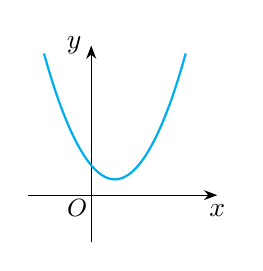
\begin{tikzpicture}[baseline={(0,0)}]
	\draw[-Stealth,name path=line](-0.8,-0.5) -- (1.6,-0.5)node[below]{$x$};
	\draw[-Stealth](0,-1.1) -- (0,1.4)node[left]{$y$};
	\draw[thick,cyan,name path=curve](-0.6,1.3) parabola bend(0.3,-0.3) (1.2,1.3);
	
	\node[below left=-3pt] at(0,-0.5){\small $O$};
	
\end{tikzpicture}
\end{document}